\documentclass[12pt, a4paper]{article}
% --- Codificación y lenguaje ---
\usepackage[utf8]{inputenc}
\usepackage[T1]{fontenc}
\usepackage[spanish]{babel}

% --- Márgenes ---
\usepackage[top=2.5cm, bottom=2.5cm, left=3cm, right=2.5cm]{geometry}

% --- Tipografía ---
\usepackage{lmodern}

% --- Matemáticas ---
\usepackage{amsmath}
\usepackage{amssymb}

% --- Figuras y tablas ---
\usepackage{graphicx}
\usepackage{booktabs}
\usepackage{float}
\usepackage{caption}
\usepackage{subcaption}

% --- Colores ---
\usepackage{xcolor}

% --- Hipervínculos ---
\usepackage[colorlinks=true, linkcolor=blue, citecolor=blue, urlcolor=blue]{hyperref}

% --- Interlineado ---
\usepackage{setspace}
\onehalfspacing

% --- Encabezados y pies de página ---
\usepackage{fancyhdr}
\pagestyle{fancy}
\fancyhf{}
\lhead{\small Teleconexiones Climáticas}
\rhead{\small Mini Proyecto 4}
\rfoot{\thepage}

% --- Bibliografía ---
\usepackage[numbers, sort&compress]{natbib}
\bibliographystyle{plainnat}

% =============================================================
\begin{document}
	
	\begin{titlepage}
		\centering
		\vspace*{2cm}
		{\LARGE \textbf{Mini Proyecto 4: Teleconexiones Climáticas en el Eje Cafetero}\\[0.5em]
			\large Variabilidad interna del sistema climático: ENSO y la Oscilación
			Multidecadal del Atlántico como moduladores de la precipitación
			y la temperatura en los Andes colombianos}\\[2cm]
		{\large Jhon García Barrera}\\[0.5em]
		{\normalsize Física del Clima y Cambio Climático}\\[0.5em]
		{\normalsize \today}\\[3cm]
		\vfill
		{\small Código y datos disponibles en:\\
			\url{https://github.com/jhongarciab/proyectos-clima/tree/main/proyecto%204}}
	\end{titlepage}
	
	\tableofcontents
	\newpage

\section{Introducción}

El clima de Colombia está determinado por una superposición de modos de variabilidad
que operan en escalas temporales muy distintas, desde la interanual hasta la
multidecadal. Comprender cómo estos modos modulan las condiciones atmosféricas locales
constituye un problema central de la climatología tropical y tiene implicaciones directas
para la gestión de recursos hídricos, la agricultura y la planificación territorial.
En este contexto, el concepto de teleconexión climática hace referencia a la
correlación estadística significativa entre anomalías climáticas en regiones geográficamente
distantes, mediada por mecanismos dinámicos de la atmósfera y el océano
\citep{Poveda1997}.

El Eje Cafetero colombiano, compuesto por los departamentos de Caldas, Risaralda y
Quindío, constituye una región de especial interés climático por varias razones.
En primer lugar, su ubicación en la vertiente occidental de la Cordillera Central de
los Andes la expone a la confluencia de tres sistemas de circulación: el chorro de
bajo nivel del Chocó, que transporta humedad desde el Pacífico oriental; el chorro
del Caribe, que aporta humedad desde el Atlántico; y la Zona de Convergencia
Intertropical (ZCIT), cuyo doble paso anual impone el régimen bimodal de
precipitación característico de la región \citep{Hoyos2018}. En segundo lugar,
la región se encuentra en la zona de transición entre la influencia del Pacífico
tropical y del Atlántico Norte, lo que la convierte en un laboratorio natural para
estudiar la competencia entre modos de variabilidad de distinto origen oceánico.

El presente trabajo explora las teleconexiones climáticas de la región del Eje
Cafetero con dos modos de variabilidad interna del sistema climático: el fenómeno
El Niño--Oscilación del Sur (ENSO, por sus siglas en inglés), representado por el
índice Niño~3.4, y la Oscilación Multidecadal del Atlántico (AMO, por sus siglas en
inglés). Ambos índices son obtenidos del repositorio de índices climáticos de la
NOAA~PSL \citep{Enfield2001, CórdobaMachado2015b}. Las variables climáticas
analizadas son la precipitación mensual y la temperatura del aire a 2~m de altura,
obtenidas del reanálisis ERA5 del Centro Europeo de Predicción Meteorológica a
Plazo Medio (ECMWF) para el período 1950--2023. La teleconexión se cuantifica
mediante la correlación cruzada de Pearson con rezago, presentando los resultados
en términos de mapas espaciales y correlogramas que permiten identificar tanto
la magnitud como el desfase temporal de las señales.

\section{Región de estudio}

El Eje Cafetero colombiano comprende los departamentos de Caldas, Risaralda y
Quindío, ubicados entre aproximadamente $3.5^\circ$N y $6^\circ$N de latitud y
$74^\circ$W y $77^\circ$W de longitud, en la vertiente occidental de la Cordillera
Central de los Andes. La región presenta una topografía altamente compleja, con
elevaciones que van desde los 800~m hasta más de 5.000~m sobre el nivel del mar en
el Nevado del Ruiz, lo que genera una marcada variabilidad espacial de temperatura
y precipitación en distancias relativamente cortas.

El régimen de precipitación es bimodal, con períodos lluviosos en marzo--mayo y
septiembre--noviembre, asociados al doble paso de la ZCIT, y períodos secos en
diciembre--febrero y junio--agosto \citep{Poveda2001}. La precipitación media anual
varía entre 1.500~mm en las zonas más altas y más de 3.000~mm en las vertientes
medias expuestas a los flujos de humedad del Pacífico. La temperatura media oscila
entre 12$^\circ$C en zonas de alta montaña y 24$^\circ$C en los valles interandinos,
con escasa variabilidad estacional pero notable variabilidad interanual asociada a
los modos de variabilidad climática de gran escala \citep{Poveda2011}.

\begin{figure}[H]
	\centering
	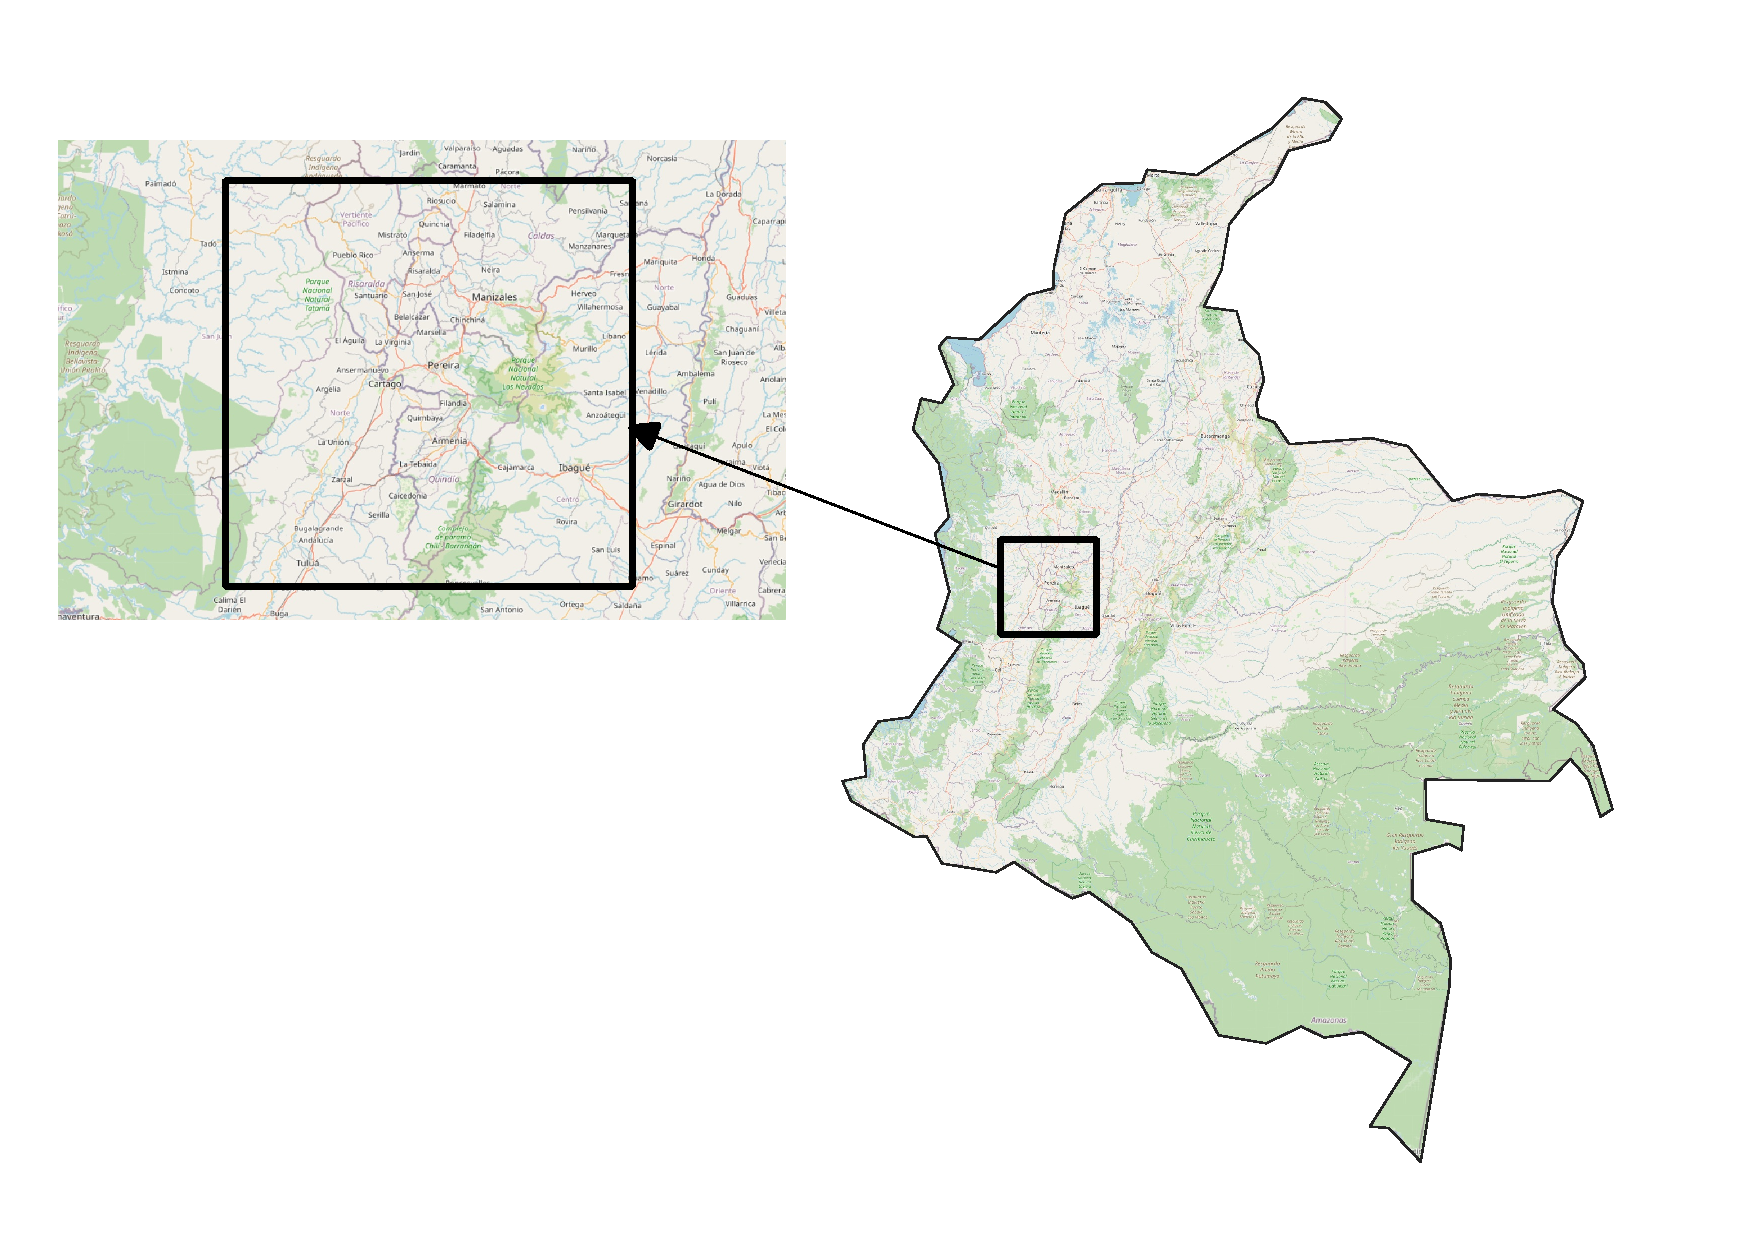
\includegraphics[width=0.65\textwidth]{../figuras/mapa.pdf}
	\caption{Localización de la región de estudio sobre
		el mapa de Colombia. La región cubre el Eje Cafetero y parte del
		departamento del Tolima, con coordenadas
		$4.0$--$5.5^{\circ}$\,N y $76.5$--$75.0^{\circ}$\,W.}
	\label{fig:mapa_region}
\end{figure}

Desde el punto de vista de la variabilidad climática, el Eje Cafetero ocupa una
posición geográfica estratégica. Al estar ubicado en el noroeste de Sudamérica,
en la transición entre la influencia del Pacífico tropical oriental y del Atlántico
Norte tropical, la región es sensible tanto al ENSO como a la AMO, aunque con
intensidades y rezagos distintos \citep{Canchala2020}. Esta dualidad de influencias
la convierte en un caso de estudio idóneo para analizar la competencia entre modos
de variabilidad de distinto origen oceánico y escala temporal. Para el análisis cuantitativo, se adoptó como punto de referencia el nodo de grilla
ERA5 más cercano a la ciudad de Armenia ($4.5^\circ$N, $75.75^\circ$W), capital del
departamento del Quindío, por ser el punto del núcleo cafetero donde la teleconexión
con el ENSO es más clara y estadísticamente robusta, con una correlación de Pearson
de $r = -0.37$ ($p < 0.001$) entre el índice Niño~3.4 y la anomalía de precipitación
mensual en rezago cero.

\section{Índices climáticos}

\subsection{ENSO: índice Niño 3.4}

El fenómeno El Niño--Oscilación del Sur (ENSO) es el modo de variabilidad
interanual dominante del sistema climático global y la principal fuente de
variabilidad hidroclimatológica en Colombia \citep{Poveda1997, Poveda2011}.
El ENSO es un fenómeno acoplado océano--atmósfera que surge de la interacción
entre las anomalías de temperatura superficial del mar (TSM) en el Pacífico
tropical y la circulación atmosférica, con una escala temporal característica
de 2 a 7 años.

El índice Niño~3.4 se construye como la anomalía de TSM promediada sobre la
región comprendida entre $5^\circ$N--$5^\circ$S y $120^\circ$--$170^\circ$W
del Pacífico central, suavizada con una media móvil de tres meses
\citep{CórdobaMachado2015b}. Valores positivos del índice indican calentamiento
anómalo del Pacífico ecuatorial central, correspondiente a la fase cálida El
Niño, mientras que valores negativos corresponden a la fase fría La Niña. La
serie utilizada en este trabajo fue obtenida del repositorio de índices
climáticos de la NOAA~PSL y cubre el período 1950--2023, con anomalías
calculadas respecto a la climatología mensual 1981--2010, presentando un rango
de $-2.38$ a $2.79$~$^\circ$C.

El mecanismo físico que conecta el ENSO con el Eje Cafetero opera principalmente
a través de la circulación de Walker. Durante la fase El Niño, el gradiente
térmico zonal del Pacífico ecuatorial se debilita, lo que reduce la convección
sobre el Pacífico oriental y genera subsidencia anómala sobre el noroeste de
Sudamérica \citep{Poveda2001}. Esta subsidencia inhibe la formación de nubes y
precipitación, produciendo déficits hídricos en la región Andina colombiana y
un calentamiento de la temperatura superficial. Durante La Niña ocurre el proceso
inverso: la intensificación de la circulación de Walker favorece la convección
y genera anomalías positivas de precipitación. Estudios previos han documentado
que el ENSO explica aproximadamente el 50\% de la variabilidad hidrológica
interanual en Colombia, con efectos más pronunciados durante diciembre--febrero
y más débiles durante marzo--mayo \citep{Poveda2011}, y con rezagos de 1 a 3
meses sobre la precipitación y el caudal \citep{CórdobaMachado2015a}.

\subsection{AMO: Oscilación Multidecadal del Atlántico}

La Oscilación Multidecadal del Atlántico (AMO) es el modo dominante de
variabilidad climática del Atlántico Norte en escalas de tiempo decadales a
multidecadales \citep{Enfield2001}. A diferencia del ENSO, que opera en escalas
interanuales, la AMO tiene una escala temporal característica de 60 a 80 años,
con una amplitud de aproximadamente $0.4^\circ$C entre sus fases extremas.

El índice AMO se construye como la media móvil de diez años de las anomalías de
TSM detrended promediadas sobre el Atlántico Norte entre $0^\circ$ y $60^\circ$N,
con el objetivo de remover la señal de tendencia asociada al calentamiento global
y aislar la variabilidad interna multidecadal \citep{Enfield2001}. En este trabajo
se utiliza la versión sin suavizar (\textit{unsmoothed}) del índice, que conserva
la variabilidad mensual real y es adecuada para el análisis de correlación en
escala mensual. La serie fue obtenida del repositorio NOAA~PSL y cubre el período
1950--2023, con un rango de $-0.54$ a $0.66^\circ$C. La AMO ha presentado una
fase negativa entre aproximadamente 1965 y 1995, y una fase positiva desde
entonces hasta el presente, como se aprecia en la serie temporal de la
Figura~\ref{fig:series}.

El mecanismo de influencia de la AMO sobre Colombia opera a través de dos vías
\citep{Knight2006, Hoyos2018}. La primera es la modulación directa de la posición
e intensidad de la ZCIT sobre el Atlántico tropical, que afecta el chorro de bajo
nivel del Caribe y la cantidad de humedad que ingresa al Eje Cafetero desde el
nororiente. La segunda es a través de teleconexiones atmosféricas que generan
anomalías de circulación sobre el noroeste de Sudamérica: durante fases positivas
de la AMO, el calentamiento del Atlántico Norte intensifica el gradiente
meridional de TSM, favoreciendo una circulación que eleva la temperatura de fondo
en los Andes tropicales \citep{DuqueGardeazabal2025}. Canchala et al.
\citep{Canchala2020} documentaron que la AMO influye sobre la precipitación en
múltiples subregiones del suroeste colombiano con rezagos de 1 a 2.5 meses,
constituyendo una teleconexión previamente subreportada en la hidroclimatología
colombiana.

\section{Datos y metodología}

\subsection{Fuentes de datos}

Los índices climáticos utilizados en este trabajo fueron obtenidos del repositorio
de índices climáticos de la Administración Nacional Oceánica y Atmosférica de los
Estados Unidos (NOAA~PSL, \url{https://psl.noaa.gov/data/climateindices/list/}).
El índice Niño~3.4 corresponde al archivo \texttt{nina34.data} y el índice AMO sin
suavizar al archivo \texttt{amon.us.data}, ambos en formato de texto plano con
resolución mensual.

Las variables climáticas fueron obtenidas del reanálisis ERA5 del Centro Europeo
de Predicción Meteorológica a Plazo Medio (ECMWF), específicamente del producto
\textit{ERA5 monthly averaged data on single levels} disponible a través del
Servicio de Cambio Climático de Copernicus (CDS). Se extrajeron dos variables:
precipitación total acumulada mensual (\texttt{tp}, en metros) y temperatura del
aire a 2~m de altura (\texttt{t2m}, en Kelvin), sobre un dominio espacial de
$3^\circ$--$7^\circ$N y $77^\circ$--$73^\circ$W con resolución de $0.25^\circ
\times 0.25^\circ$, resultando en una grilla de $17 \times 17$ puntos. La
precipitación fue convertida a mm~mes$^{-1}$ multiplicando por 1000, y la
temperatura a grados Celsius restando 273.15~K. El período de análisis cubre
enero de 1950 a diciembre de 2023, totalizando 888 meses.

\subsection{Procesamiento}

Las anomalías mensuales de precipitación y temperatura ERA5 se calcularon
restando la climatología mensual del período de referencia 1981--2010, siguiendo
la convención estándar de la Organización Meteorológica Mundial. Las anomalías
del índice Niño~3.4 se obtuvieron restando la media climatológica mensual del
mismo período de referencia, obteniéndose una serie con rango de $-2.38$ a
$2.79^\circ$C. El índice AMO sin suavizar ya representa anomalías detrended y
no requirió procesamiento adicional, con un rango de $-0.54$ a $0.66^\circ$C.
El período común de análisis para los cuatro conjuntos de datos es enero de
1950 a diciembre de 2023 (888 meses).

\subsection{Cuantificador: correlación cruzada de Pearson rezagada}

La teleconexión entre cada índice climático y cada variable ERA5 se cuantificó
mediante la correlación cruzada de Pearson con rezago, definida como:

\begin{equation}
	r(\tau) = \frac{\displaystyle\sum_{t=1}^{N-\tau}
		\bigl[X(t) - \bar{X}\bigr]\bigl[Y(t+\tau) - \bar{Y}\bigr]}
	{\displaystyle\sqrt{\sum_{t=1}^{N-\tau}\bigl[X(t)-\bar{X}\bigr]^2\;
			\sum_{t=1}^{N-\tau}\bigl[Y(t+\tau)-\bar{Y}\bigr]^2}}
	\label{eq:pearson}
\end{equation}

\noindent donde $X(t)$ es la serie del índice climático, $Y(t+\tau)$ es la
serie de la variable ERA5 en el tiempo $t+\tau$, $\tau$ es el rezago en meses
(con $\tau > 0$ indicando que el índice lidera a la variable), y $N = 888$ es
la longitud total de la serie. El cálculo se realizó para rezagos
$\tau \in \{0, 1, 2, \ldots, 12\}$ meses y para cada uno de los $17 \times 17$
puntos de grilla del dominio, generando mapas espaciales de correlación para
cada rezago y cada par índice--variable.

\subsection{Significancia estadística}

La significancia estadística de cada coeficiente de correlación se evaluó
mediante el test de Student bilateral, con umbral $p < 0.05$. Para una muestra
de $N$ observaciones, el estadístico de prueba es:

\begin{equation}
	t = r\sqrt{\frac{N-2}{1-r^2}}
	\label{eq:ttest}
\end{equation}

\noindent que sigue una distribución $t$ de Student con $N-2$ grados de
libertad bajo la hipótesis nula $H_0: r = 0$. El valor crítico de correlación
para $p < 0.05$ con $N = 888$ es $r_{\text{crit}} \approx \pm 0.066$.
Las regiones donde la correlación no supera este umbral se indican en los mapas
mediante sombreado con rayas diagonales. Cabe señalar que este umbral asume
independencia entre observaciones sucesivas, supuesto que puede ser violado en
series climáticas con autocorrelación significativa \citep{Wilks2011}; sin
embargo, dado que se trabaja con anomalías mensuales sobre un período de 74 años,
el número efectivo de grados de libertad permanece elevado y el efecto sobre el
umbral de significancia es moderado.

\section{Resultados}

\subsection{Series temporales de los índices y las variables climáticas}

La Figura~\ref{fig:series} muestra las series temporales mensuales del índice
Niño~3.4 (anomalía de TSM), el índice AMO, y las anomalías de precipitación y
temperatura a 2~m en el punto de referencia de Armenia ($4.5^\circ$N,
$75.75^\circ$W) para el período 1950--2023.

\begin{figure}[H]
	\centering
	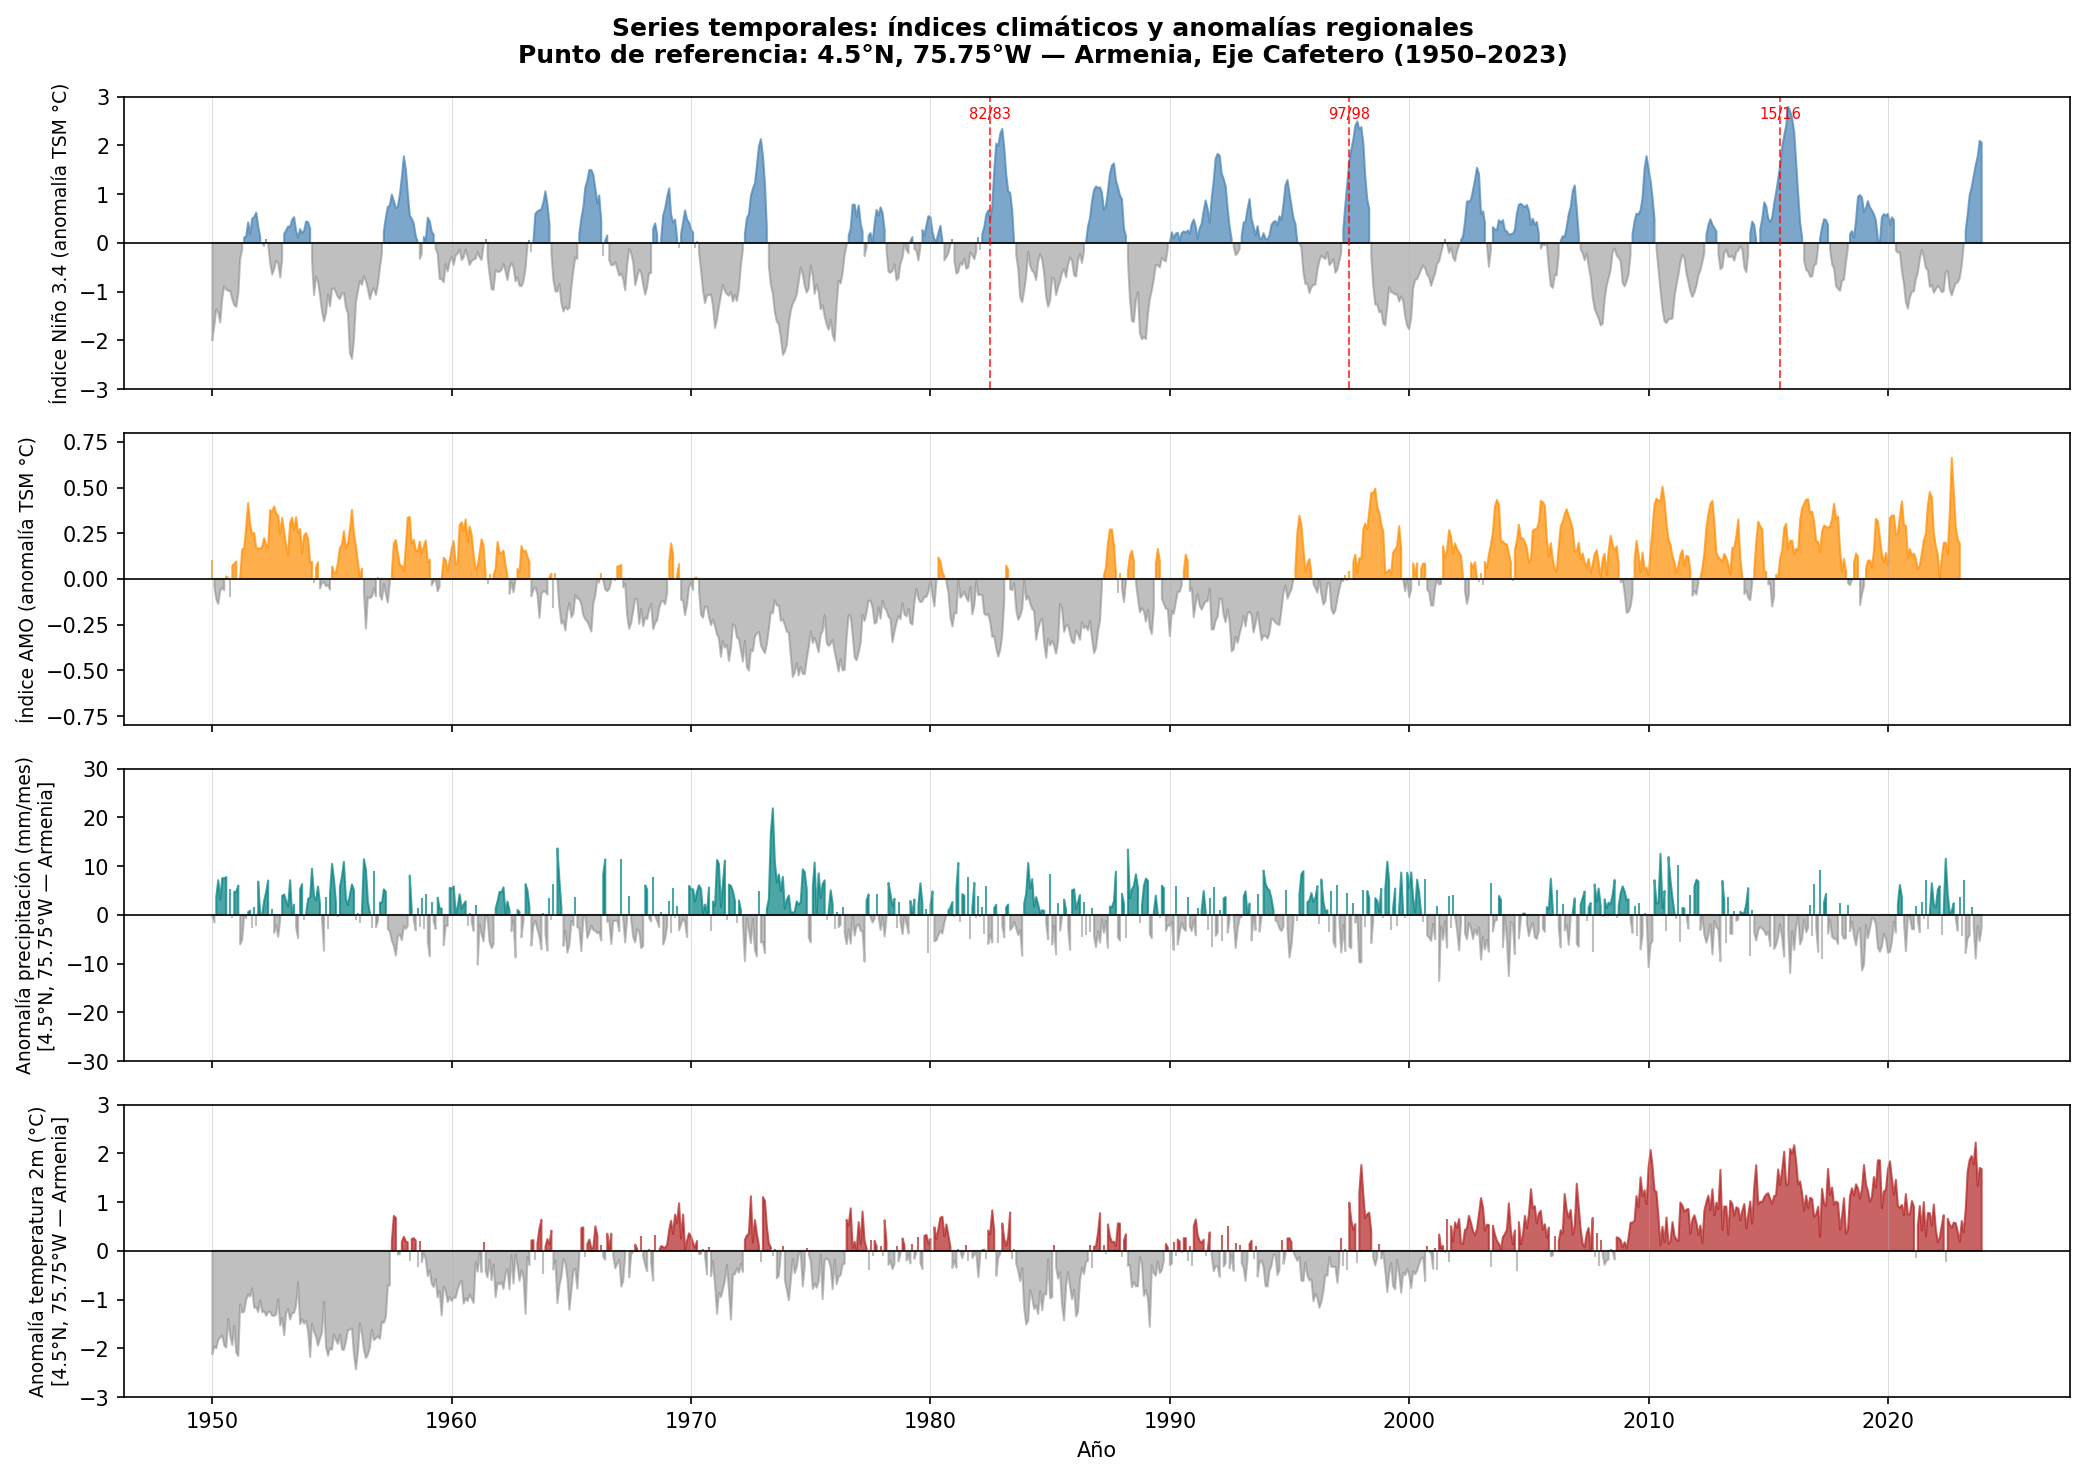
\includegraphics[width=0.75\textwidth]{../figuras/fig2_series_temporales.png}
	\caption{Series temporales mensuales de los índices climáticos y las
		anomalías de las variables ERA5 en el punto de referencia
		($4.5^\circ$N, $75.75^\circ$W, Armenia). De arriba a abajo: anomalía
		de TSM del índice Niño~3.4 ($^\circ$C), índice AMO ($^\circ$C),
		anomalía de precipitación (mm~mes$^{-1}$) y anomalía de temperatura
		a 2~m ($^\circ$C). Las líneas verticales rojas señalan los eventos
		El Niño fuertes de 1982/83, 1997/98 y 2015/16. El color indica signo
		positivo (color sólido) o negativo (gris).}
	\label{fig:series}
\end{figure}

El índice Niño~3.4 exhibe la variabilidad interanual característica del ENSO,
con eventos El Niño claramente identificables en 1957, 1965, 1972, 1982, 1987,
1997 y 2015, y episodios La Niña pronunciados en 1955, 1970, 1973, 1988 y 1999.
El índice AMO muestra el comportamiento multidecadal esperado \citep{Enfield2001,
	Knight2006}: una fase positiva durante 1950--1963, una transición a fase negativa
entre 1964 y aproximadamente 1995, y una fase positiva sostenida desde entonces
hasta el presente, con valores que superan los $0.5^\circ$C a partir de 2010.

La anomalía de temperatura a 2~m en Armenia exhibe una tendencia al calentamiento
progresiva y estadísticamente visible a partir de la década de 2000, consistente
con la superposición de la fase positiva de la AMO y el calentamiento de fondo
asociado al cambio climático \citep{Poveda2011}. La anomalía de precipitación
presenta variabilidad interanual con amplitud de $\pm 14$~mm~mes$^{-1}$, sin
una tendencia temporal clara, lo que sugiere que la precipitación en este punto
está controlada principalmente por la variabilidad interna y no por un forzamiento
externo de baja frecuencia dominante.

\subsection{Mapas de correlación rezagada}

La Figura~\ref{fig:mapas} presenta los mapas de correlación de Pearson entre
cada índice climático y cada variable ERA5, evaluados en el rezago de máxima
coherencia física identificado en el análisis de correlación cruzada.

\begin{figure}[H]
	\centering
	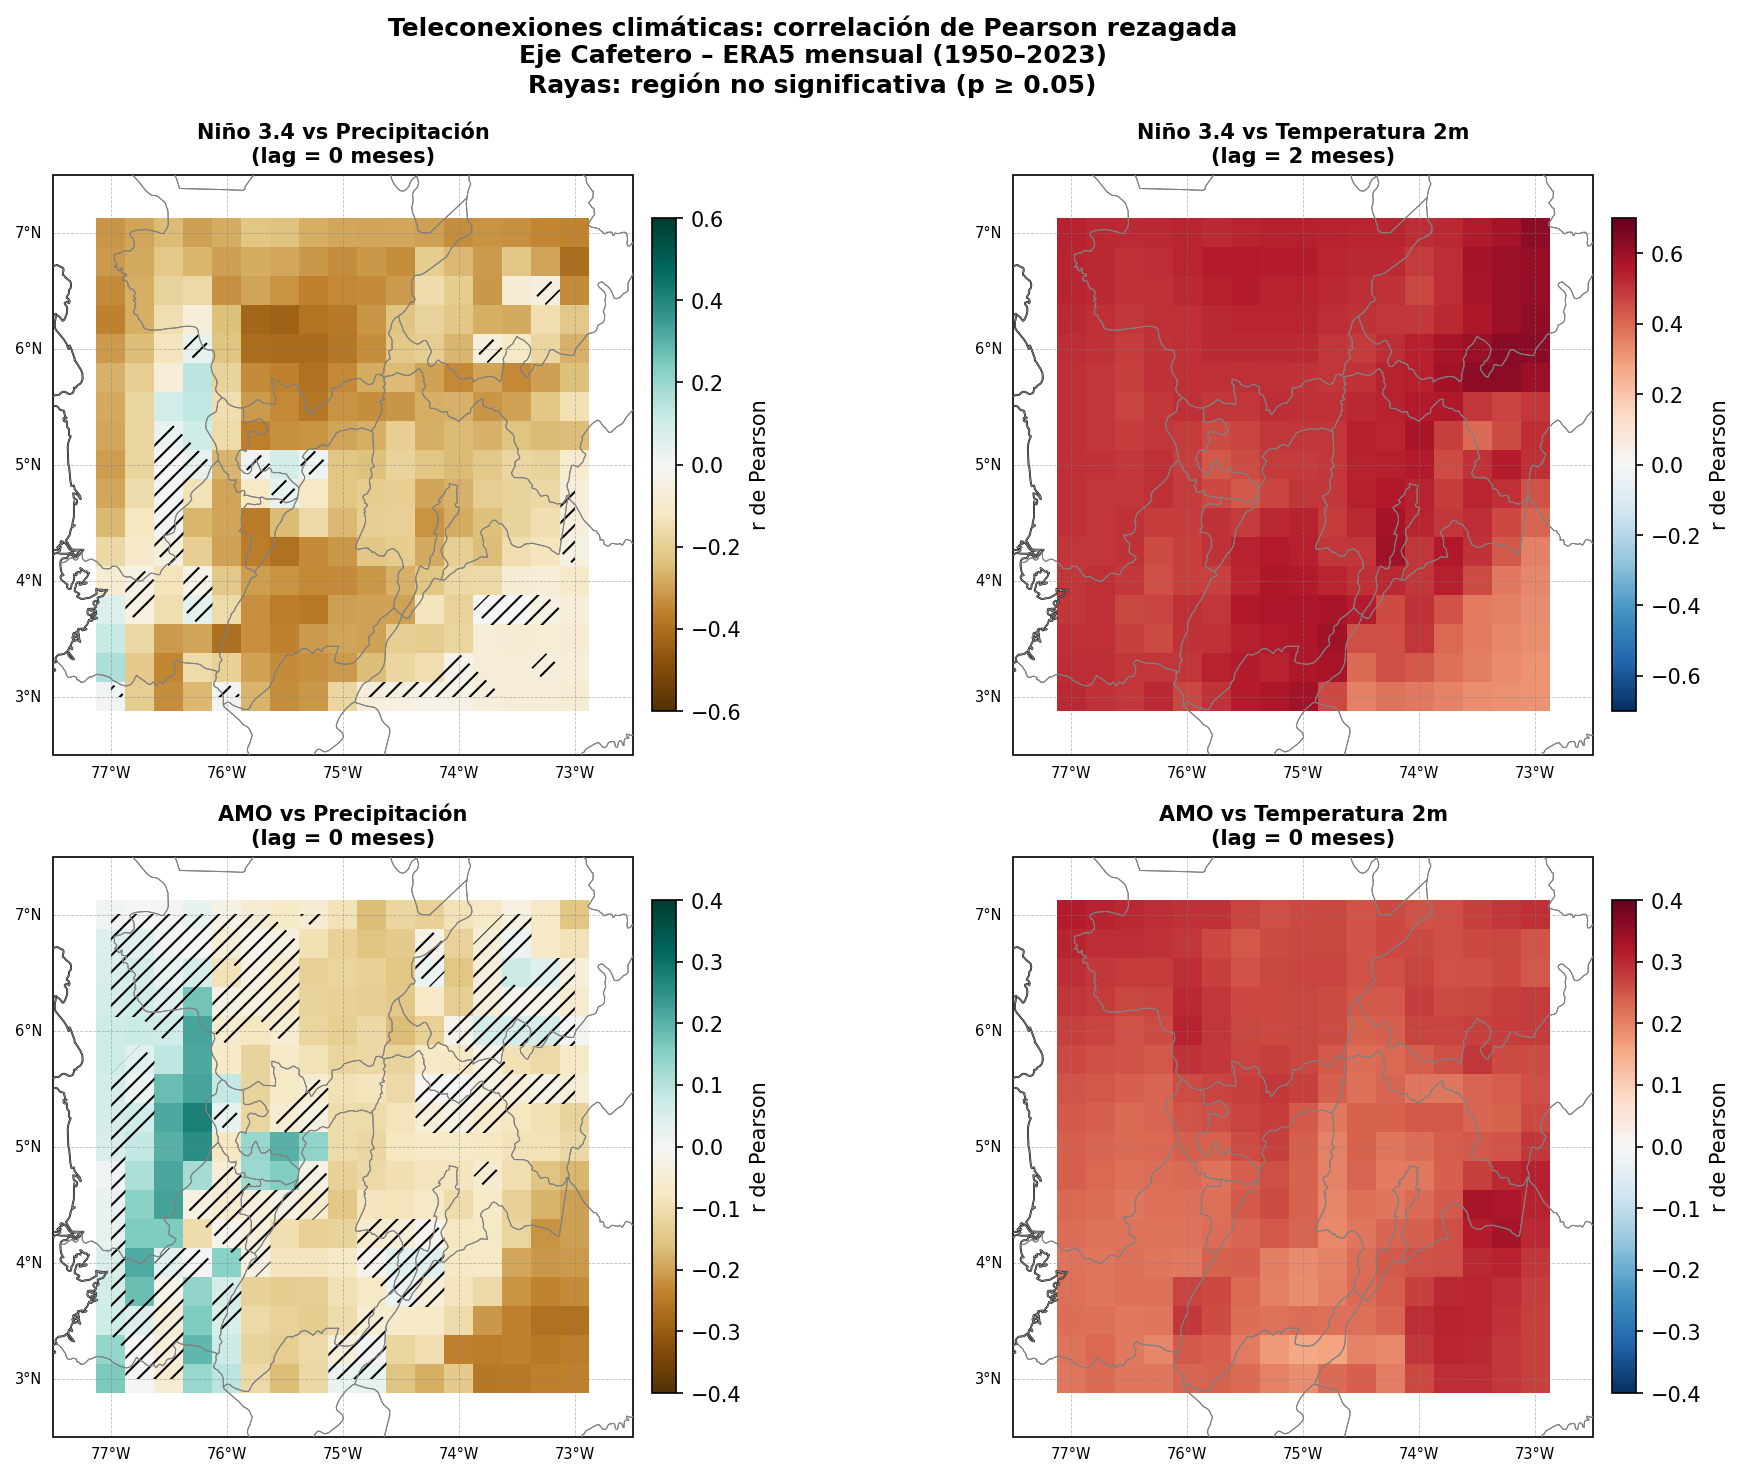
\includegraphics[width=0.75\textwidth]{../figuras/fig1_mapas_correlacion.png}
	\caption{Mapas de correlación de Pearson entre los índices climáticos y las
		variables ERA5 sobre el Eje Cafetero (1950--2023). Superior izquierda:
		Niño~3.4 vs precipitación (lag~$= 0$ meses). Superior derecha: Niño~3.4
		vs temperatura 2~m (lag~$= 2$ meses). Inferior izquierda: AMO vs
		precipitación (lag~$= 0$ meses). Inferior derecha: AMO vs temperatura 2~m
		(lag~$= 0$ meses). Las rayas diagonales indican regiones donde la
		correlación no es estadísticamente significativa ($p \geq 0.05$).}
	\label{fig:mapas}
\end{figure}

El panel superior izquierdo muestra que el índice Niño~3.4 se correlaciona
negativamente con la precipitación en la mayor parte del Eje Cafetero en lag~$=0$,
con valores de $r$ entre $-0.2$ y $-0.4$ en el núcleo de la región. Esta señal
es físicamente coherente con el mecanismo de subsidencia anómala documentado por
\citet{Poveda1997} y \citet{Poveda2001}: durante El Niño, la debilitación de la
circulación de Walker genera subsidencia sobre el noroeste de Sudamérica que inhibe
la convección y reduce la precipitación. La correlación es heterogénea espacialmente,
con zonas no significativas al occidente, correspondientes al corredor del Pacífico
donde la precipitación está controlada principalmente por el chorro del Chocó y
es menos sensible al ENSO \citep{Hoyos2018}.

El panel superior derecho revela la teleconexión más robusta del análisis: el
índice Niño~3.4 se correlaciona positivamente con la temperatura a 2~m en
lag~$= 2$ meses, con valores de $r$ entre $0.4$ y $0.7$ en prácticamente toda
la región, y con muy pocas zonas no significativas. Este resultado indica que
El Niño calienta el Eje Cafetero con un rezago de 2 meses respecto a la
anomalía de TSM en el Pacífico central, consistente con los tiempos de propagación
de la señal atmosférica documentados por \citet{CórdobaMachado2015a}.

Los paneles inferiores muestran las teleconexiones de la AMO. La correlación
con la precipitación (inferior izquierda) es débil y espacialmente heterogénea,
con amplias zonas no significativas, lo que refleja la naturaleza de baja
frecuencia de este índice y su escasa influencia directa sobre la precipitación
mensual. La correlación con la temperatura (inferior derecha) es positiva y
significativa en la mayor parte de la región ($r \approx 0.2$--$0.3$), indicando
que las fases cálidas de la AMO se asocian con temperaturas más altas en el Eje
Cafetero, resultado consistente con los hallazgos de \citet{DuqueGardeazabal2025}
sobre la influencia del Atlántico en la variabilidad térmica del noroeste de
Sudamérica.

\subsection{Correlación cruzada en función del rezago}

La Figura~\ref{fig:correlograma} muestra el correlograma de correlación cruzada
para los cuatro pares índice--variable en el punto de referencia de Armenia,
evaluado para rezagos entre $-12$ y $+12$ meses.

El correlograma Niño~3.4 vs precipitación (panel superior izquierdo) muestra
una estructura asimétrica: la correlación es negativa y significativa para
rezagos de $-12$ a $0$ meses, con un máximo absoluto en lag~$= -2$
($r = -0.34$), lo que indica que la precipitación en Armenia responde
rápidamente a las anomalías del Pacífico. La correlación se vuelve no
significativa para rezagos positivos mayores a 1 mes, consistente con la
escala temporal interanual del ENSO y la naturaleza transitoria de su impacto
sobre la precipitación local \citep{Poveda2001}.
El correlograma Niño~3.4 vs temperatura (panel superior derecho) exhibe la
señal más clara y persistente del análisis: la correlación es positiva y
significativa para todos los rezagos entre $-9$ y $+12$ meses, con un máximo
en lag~$= 2$ ($r = 0.50$). Esta persistencia refleja la inercia térmica de la
atmósfera andina y el carácter sostenido de los eventos ENSO, que típicamente
se prolongan por 12 a 18 meses \citep{Poveda2011}.

El correlograma AMO vs precipitación (panel inferior izquierdo) muestra
correlaciones negativas y débiles ($r \approx -0.21$) principalmente para
rezagos negativos, sin una estructura de rezago clara, lo que es consistente
con la naturaleza de baja frecuencia de la AMO y su escasa influencia directa
sobre la precipitación mensual \citep{Canchala2020}.

\begin{figure}[H]
	\centering
	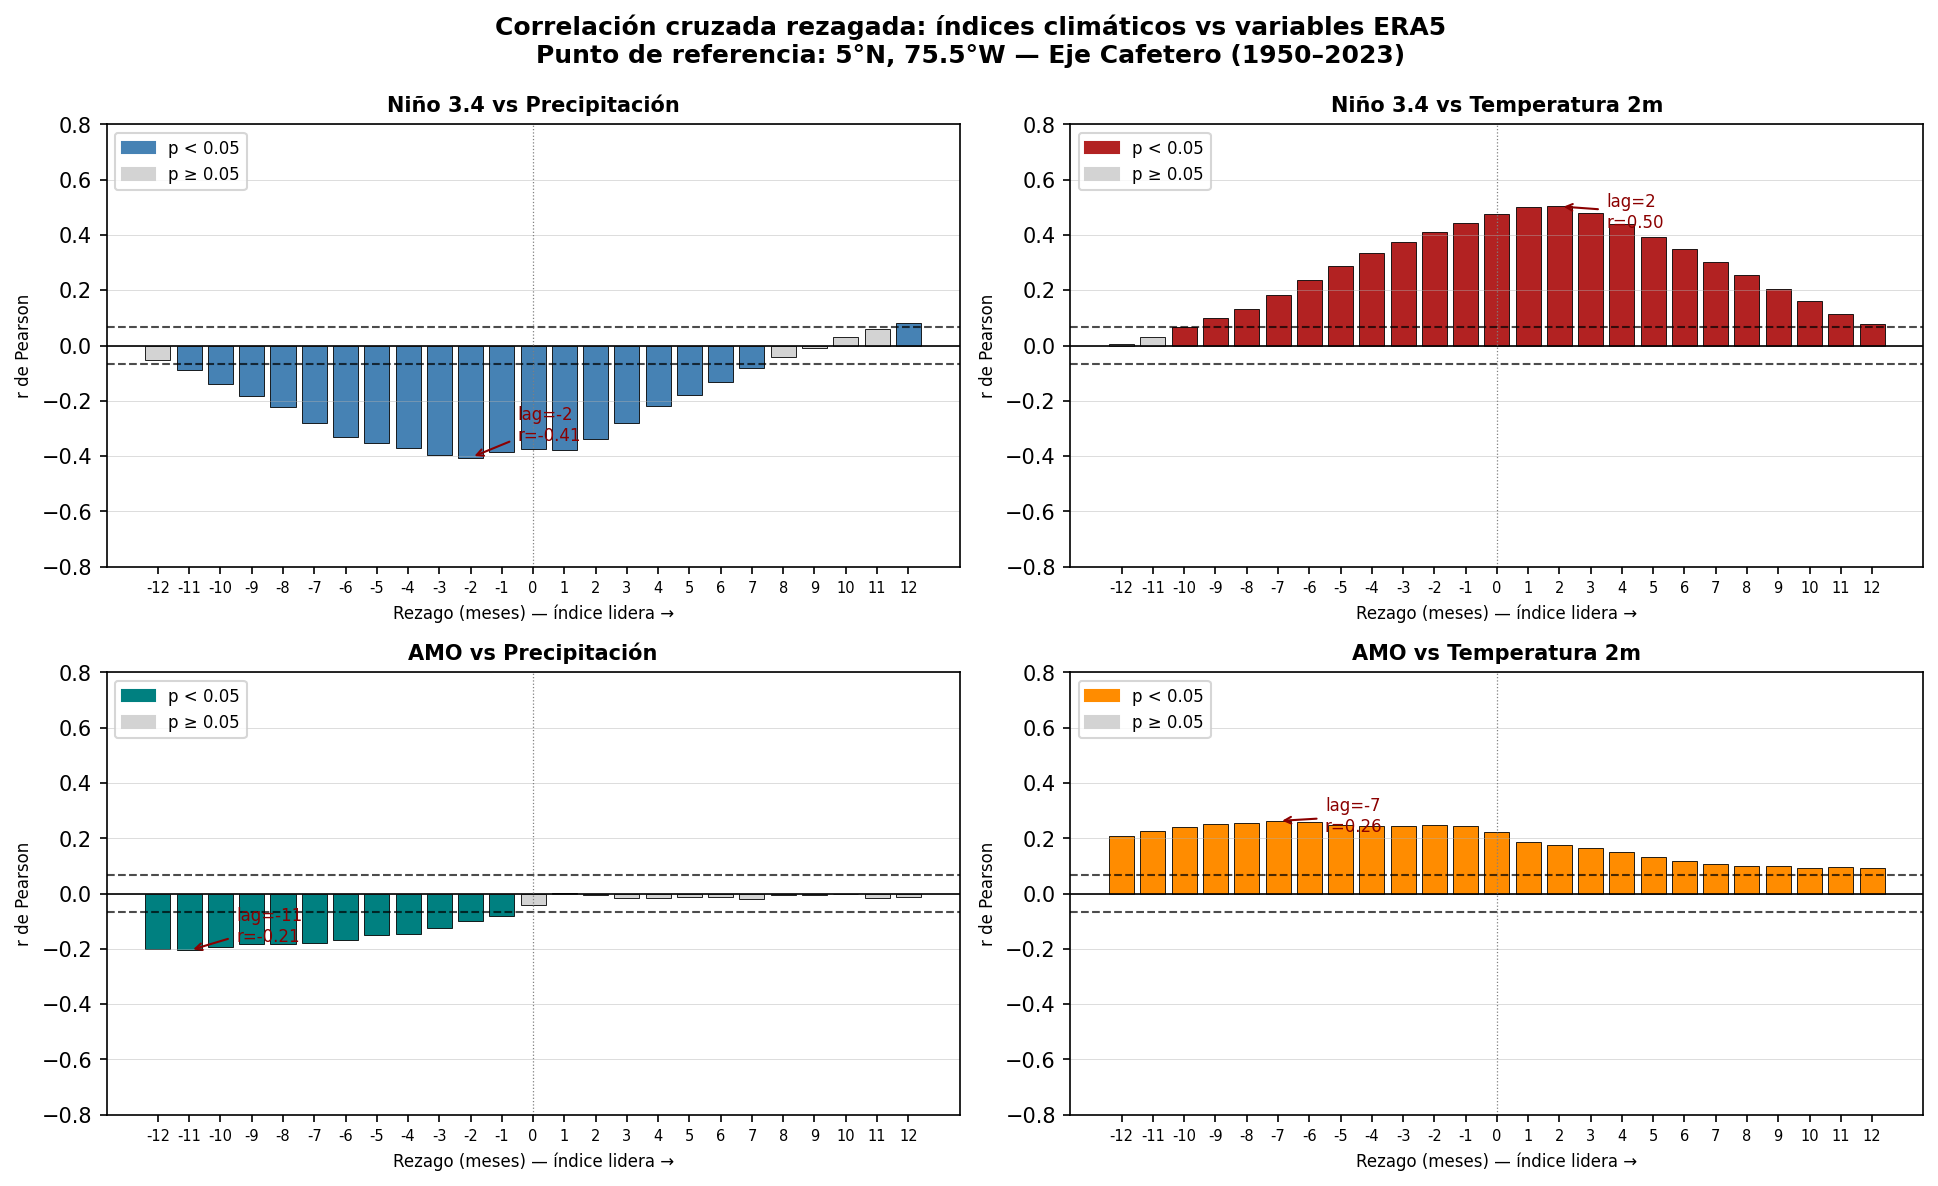
\includegraphics[width=0.70\textwidth]{../figuras/fig3_correlograma.png}
	\caption{Correlación cruzada de Pearson en función del rezago (meses) entre
		los índices climáticos y las variables ERA5 en el punto de referencia
		($4.5^\circ$N, $75.75^\circ$W). Rezagos positivos indican que el índice
		lidera a la variable. Las barras de color indican correlaciones
		estadísticamente significativas ($p < 0.05$) y las barras grises
		correlaciones no significativas. Las líneas discontinuas horizontales
		muestran el umbral de significancia $r_{\text{crit}} = \pm 0.066$.
		La anotación en rojo indica el rezago de máxima correlación absoluta.}
	\label{fig:correlograma}
\end{figure}

Finalmente, el correlograma AMO vs temperatura (panel inferior derecho) muestra
una correlación positiva persistente ($r \approx 0.2$--$0.26$) y prácticamente
plana en todos los rezagos evaluados. Esta estructura es característica de un
forzante de baja frecuencia: la AMO modula la temperatura de fondo del Eje
Cafetero sin un rezago temporal definido, actuando como una señal de lenta
variación sobre la cual se superpone la variabilidad interanual del ENSO
\citep{Knight2006, DuqueGardeazabal2025}.

\section{Discusión}

Los resultados presentados en la sección anterior permiten identificar dos
regímenes de teleconexión cualitativamente distintos sobre el Eje Cafetero:
uno de carácter interanual, dominado por el ENSO, y otro de carácter
multidecadal, asociado a la AMO. La superposición de ambos modos sobre las
variables climáticas locales es coherente con el marco teórico de la
variabilidad climática interna descrito por \citet{Poveda2011} y
\citet{Canchala2020}.

\subsection{Teleconexión ENSO--Eje Cafetero}

La señal ENSO más robusta del análisis corresponde a la temperatura a 2~m,
con $r = 0.50$ en lag~$= 2$ meses. Este resultado es consistente con la
literatura: \citet{Poveda1997} y \citet{Poveda2001} documentaron que durante
El Niño la región Andina colombiana experimenta anomalías positivas de
temperatura superficial asociadas a la reducción de la cobertura nubosa y el
aumento de la radiación de onda corta en superficie, consecuencia directa de
la subsidencia anómala generada por el debilitamiento de la circulación de
Walker. El rezago de 2 meses es consistente con los tiempos de propagación
de la señal atmosférica desde el Pacífico central hasta los Andes colombianos
documentados por \citet{CórdobaMachado2015a}, quienes reportaron rezagos de
1 a 3 meses para la mayor parte de las variables hidroclimatológicas de
Colombia.

La señal ENSO sobre la precipitación es más débil ($r = -0.37$ en lag~$= 0$
en Armenia) y espacialmente heterogénea. Esta moderada magnitud de la
correlación es un hallazgo esperado y no constituye una anomalía del análisis.
El Eje Cafetero se ubica en la zona de transición entre la influencia del
Pacífico y del Atlántico, lo que diluye la señal ENSO respecto a regiones
más claramente dominadas por uno u otro océano \citep{Hoyos2018}. Además,
la precipitación en la región está fuertemente controlada por factores
topográficos locales y por el ciclo diurno de la convección, que introducen
variabilidad de alta frecuencia no relacionada con el ENSO y que el reanálisis
ERA5 en resolución de $0.25^\circ$ captura solo parcialmente. \citet{Poveda2011}
reportaron que el ENSO explica aproximadamente el 50\% de la variabilidad
hidrológica interanual en Colombia, pero con diferencias regionales
significativas: la influencia es más pronunciada en la región Caribe y
Andina norte, y más débil en las vertientes orientales donde el régimen
amazónico tiene mayor peso.

La heterogeneidad espacial observada en el mapa de correlación Niño~3.4 vs
precipitación merece atención particular. Las zonas con correlaciones no
significativas al occidente del dominio corresponden al corredor del Pacífico
colombiano, donde la precipitación está controlada principalmente por el chorro
de bajo nivel del Chocó \citep{Hoyos2018}. Este chorro, que transporta humedad
desde el Pacífico oriental ecuatorial hacia el interior del continente, no
responde de manera simple al ENSO: aunque El Niño debilita la convección en el
Pacífico ecuatorial central, el Pacífico oriental ecuatorial puede mantener o
incluso intensificar su actividad convectiva en algunos eventos, generando
respuestas de precipitación no monótonas en esta zona \citep{CórdobaMachado2015a}.

\subsection{Teleconexión AMO--Eje Cafetero}

La AMO exhibe una influencia más clara sobre la temperatura ($r \approx 0.25$)
que sobre la precipitación ($r \approx -0.10$ a $-0.20$) en el Eje Cafetero.
La correlación AMO--temperatura es positiva, persistente en todos los rezagos
evaluados y significativa en la mayor parte de la región, lo que es consistente
con el mecanismo propuesto por \citet{Knight2006}: durante las fases positivas
de la AMO, el calentamiento del Atlántico Norte intensifica el transporte de
calor hacia el trópico y eleva la temperatura de fondo de la atmósfera tropical,
incluyendo los Andes colombianos. \citet{DuqueGardeazabal2025} demostraron
que la influencia atlántica sobre la evapotranspiración y la temperatura en
las cuencas del Orinoco y Amazonas, adyacentes al Eje Cafetero, opera a través
de este mecanismo de calentamiento de fondo.

La señal AMO sobre la precipitación es débil y espacialmente incoherente, con
amplias zonas no significativas en los mapas. Este resultado es esperable por
dos razones. Primero, la AMO opera en escalas de 60 a 80 años \citep{Enfield2001},
de modo que su varianza mensual es pequeña comparada con la del ENSO, y su
señal sobre la precipitación mensual queda enmascarada por la variabilidad de
alta frecuencia. Segundo, el período de análisis de 74 años cubre menos de dos
ciclos completos de la AMO, lo que limita el poder estadístico para detectar su
influencia sobre variables de alta variabilidad como la precipitación. Esta
limitación es intrínseca a cualquier análisis de teleconexiones multidecadales
con registros instrumentales de longitud finita \citep{Canchala2020}.

\subsection{Interacción entre ENSO y AMO}

Un aspecto que los resultados sugieren, aunque no se cuantifica explícitamente
en este trabajo, es la posible interacción entre ambos modos de variabilidad.
La AMO, al modular la temperatura de fondo del Eje Cafetero, puede amplificar
o atenuar el impacto térmico del ENSO: durante la fase positiva actual de la
AMO (desde ~1995), los eventos El Niño generan anomalías de temperatura más
pronunciadas que en la fase negativa anterior, porque parten de una línea base
más cálida. Esta hipótesis es consistente con la tendencia al calentamiento
visible en la serie temporal de la Figura~\ref{fig:series} a partir de 2000,
y con los hallazgos de \citet{Poveda2011} sobre la modulación multidecadal
de los impactos del ENSO en Colombia. La cuantificación explícita de esta
interacción requeriría un análisis de correlación parcial o de correlación
condicional a la fase de la AMO, lo que constituye una extensión natural de
este trabajo.

\subsection{Limitaciones metodológicas}

El análisis presentado tiene tres limitaciones que deben considerarse en la
interpretación de los resultados. Primera, la correlación de Pearson asume
una relación lineal entre los índices y las variables climáticas, supuesto
que puede ser violado dado que la respuesta hidrológica al ENSO en Colombia
es conocidamente no lineal, con asimetrías entre El Niño y La Niña
\citep{Poveda2011, CórdobaMachado2015a}. Segunda, el test de significancia estándar asume
independencia entre observaciones, mientras que las series climáticas mensuales
presentan autocorrelación significativa que reduce el número efectivo de grados
de libertad; aunque el efecto es moderado con 888 observaciones, un análisis
riguroso
debería corregir el umbral de significancia por autocorrelación
siguiendo el procedimiento descrito por Wilks \citet{Wilks2011} en el capítulo~3
del texto de referencia del curso. Tercera, el
análisis se limita a un dominio espacial reducido ($3^\circ$--$7^\circ$N,
$77^\circ$--$73^\circ$W) centrado en el Eje Cafetero, lo que impide visualizar
el patrón de teleconexión en su contexto continental más amplio, como el
presentado por \citet{CórdobaMachado2015b} para toda Colombia.

\section{Conclusiones}

Este trabajo analizó las teleconexiones climáticas del Eje Cafetero colombiano
con dos modos de variabilidad interna del sistema climático: el ENSO, representado
por el índice Niño~3.4, y la Oscilación Multidecadal del Atlántico (AMO), para
el período 1950--2023. El análisis de correlación cruzada de Pearson rezagada
entre los índices NOAA~PSL y las anomalías de precipitación y temperatura a 2~m
del reanálisis ERA5 permite extraer las siguientes conclusiones:

\begin{enumerate}
	
	\item El ENSO es el modo de variabilidad interna con mayor influencia sobre
	el Eje Cafetero en escala interanual. Su teleconexión más robusta corresponde
	a la temperatura a 2~m, con una correlación de Pearson de $r = 0.50$ en un
	rezago de 2 meses ($p < 0.001$), estadísticamente significativa en la casi
	totalidad del dominio espacial analizado. Durante El Niño, la subsidiencia
	anómala generada por el debilitamiento de la circulación de Walker produce
	un calentamiento de la región con un desfase de aproximadamente dos meses
	respecto a la anomalía de TSM en el Pacífico central \citep{Poveda1997,
		CórdobaMachado2015a}.
	
	\item La teleconexión ENSO--precipitación es significativa pero moderada
	($r = -0.37$ en lag~$= 0$ en el punto de referencia de Armenia), con
	heterogeneidad espacial marcada. Las zonas de correlación no significativa
	al occidente del dominio corresponden al corredor del Pacífico colombiano,
	donde la precipitación está controlada por el chorro del Chocó y responde
	de manera menos directa al ENSO \citep{Hoyos2018}. Esta moderada magnitud
	es consistente con la posición del Eje Cafetero en la zona de transición
	entre la influencia del Pacífico y del Atlántico \citep{Poveda2011}.
	
	\item La AMO ejerce una influencia significativa sobre la temperatura del
	Eje Cafetero ($r \approx 0.25$, $p < 0.05$ en la mayor parte del dominio),
	con una estructura de correlación plana en todos los rezagos evaluados,
	característica de un forzante de baja frecuencia que modula la temperatura
	de fondo sin un desfase temporal definido \citep{Knight2006,
		DuqueGardeazabal2025}. La fase positiva de la AMO desde aproximadamente
	1995 es consistente con la tendencia al calentamiento progresivo observada
	en la serie temporal de temperatura del punto de referencia.
	
	\item La influencia de la AMO sobre la precipitación mensual es débil y
	estadísticamente no significativa en la mayor parte del dominio, resultado
	esperable dado que la AMO opera en escalas de 60 a 80 años y su varianza
	mensual queda enmascarada por la variabilidad de alta frecuencia de la
	precipitación local \citep{Enfield2001, Canchala2020}.
	
	\item Los dos modos de variabilidad actúan en escalas temporales distintas
	y complementarias: el ENSO domina la variabilidad interanual de ambas
	variables, mientras que la AMO modula la temperatura de fondo en escala
	multidecadal. Su superposición sugiere que los impactos térmicos del ENSO
	sobre la región pueden ser amplificados durante la fase positiva actual de
	la AMO, hipótesis que constituye una extensión natural de este trabajo
	mediante análisis de correlación parcial o condicional.
	
\end{enumerate}

En conjunto, los resultados confirman la relevancia de considerar múltiples
modos de variabilidad climática interna para caracterizar el clima del Eje
Cafetero, y subrayan la utilidad del análisis de correlación rezagada como
herramienta para identificar teleconexiones en escala mensual. Futuros trabajos
podrían extender el dominio espacial al conjunto de Colombia para comparar
la estructura de las teleconexiones entre regiones, incorporar cuantificadores
no lineales como la transferencia de entropía para capturar asimetrías entre
fases del ENSO \citep{Poveda2011,
	CórdobaMachado2015a}, o explorar la interacción explícita entre
ENSO y AMO mediante análisis de correlación condicional a la fase del índice
multidecadal.

\bibliography{referencias_miniproyecto4}

\end{document}
